\bookchapter{第六十章：開発環境を整える——Xcodeと最初のプロジェクト}

\chapterintro{仕事をうまくやるには、まず道具をととのえること。この章では「キッチン」を整えます：Xcodeを入れて、シミュレータを動かして、人生初のiOSプロジェクトを作り、さらにプロジェクトの構造をばらして丸ごと理解します。環境が整えば、自分が書いたコードが「押せるボタン」になる瞬間に初めて出会えます——この瞬間を一生覚えている人は多いものです。}

\booksection{Macを1台用意する}

まずハードルの話：iOS開発はmacOS上で行う必要があります。Macを持っていない場合、選択肢は3つ。1台買う（中古のMac miniやMacBook Airでも十分）、短期だけクラウドMacを借りる、あるいは先に第8編『Android開発実践編』（WindowsでOK）を読む——この3つです。

\begin{center}
\begin{tabularx}{\linewidth}{|X|X|X|}
\hline
\textbf{項目} & \textbf{最低要件} & \textbf{快適ライン（おすすめ）} \tabularnewline
\hline
チップ & Apple Silicon（M1以降） & M2以降 \tabularnewline
メモリ & 8GB & 16GB \tabularnewline
ストレージ & 40GB以上を確保（Xcode本体はかなり大きい） & 256GB以上 \tabularnewline
OS & 最新のmacOS & 自動更新をオンのまま \tabularnewline
\hline
\end{tabularx}
\end{center}

\begin{center}\small\color{gray}Mac開発マシンの構成目安（2026年8月）\end{center}

\begin{tcbinfo}{ワンポイント：Macがなくても、言語から先に学べる}
iPadの無料アプリSwift Playgroundsなら、MacなしでSwiftの基礎が学べます（iPhoneにも入れます）。まず第六十一章の言語の知識をPlaygroundsで遊びながら慣らしておき、Macを手に入れたらそのまま飛び立てます。「薪を割る前に斧を研ぐ時間は無駄にならない」というわけです。

\end{tcbinfo}

\booksection{Xcodeをインストールする}

XcodeはApple公式の統合開発環境で、無料です。3ステップで入れましょう：

\begin{enumerate}
  \item MacでApp Storeを開き、「Xcode」と検索してインストールをクリック——数GBあるので、ネットが快適な時間帯を選びましょう。
  \item インストール後の初回起動で規約に同意し、必要なコンポーネントを入れます（自動で完了します）。
  \item メニューのXcode Settings Locationsで、Command Line Toolsが選択されているか確認します——コマンドラインツールは、多くのスクリプトやサードパーティツールの前提になるものです。
\end{enumerate}

\begin{tcbwarn}{注意：バージョンとOSの「組み合わせゲーム」}
新しいXcodeはたいてい最新のmacOSを求め、古いMacは古いバージョンで止まってしまいます。App Storeに公開するとき、Appleは比較的新しいXcodeでのビルドを求めます（たいてい猶予期間はあります）。だからOSの更新はサボらないでください——iOS開発者は「最新版を追いかける」のがいちばん勤勉な集団なのです。

\end{tcbwarn}

\booksection{最初のプロジェクトを作る}

Xcodeを開いてCreate New Project iOSを選択 Appテンプレートを選び、次のように入力します：

\begin{center}
\begin{tabularx}{\linewidth}{|X|X|X|}
\hline
\textbf{項目} & \textbf{入力するもの} & \textbf{説明} \tabularnewline
\hline
Product Name & MyFirstApp & アプリ名 \tabularnewline
Team & あなたのApple ID（無料） & 署名用。個人アカウントでOK \tabularnewline
Organization Identifier & com.example & Product Nameと組み合わせてパッケージIDになる \tabularnewline
Interface & SwiftUI & 本書のメインで使うフレームワーク \tabularnewline
Language & Swift & 説明は不要でしょう \tabularnewline
\hline
\end{tabularx}
\end{center}

\begin{center}\small\color{gray}プロジェクト作成で入力する5つの項目\end{center}

Createを押すと、Xcodeはそのまま実行できるプロジェクトを生成します。左上でシミュレータを1台選び（たとえばiPhone 17）、>を押して実行——数秒後、シミュレータの画面に「Hello, world!」と書かれたウィンドウが現れます。あなたの初めてのiOSアプリが誕生した瞬間です。

\booksection{プロジェクト構造の分解：ファイルごとの役割}

左側はプロジェクトナビゲータです。初心者がまず知っておけばいいのはこのくらい：

\begin{center}
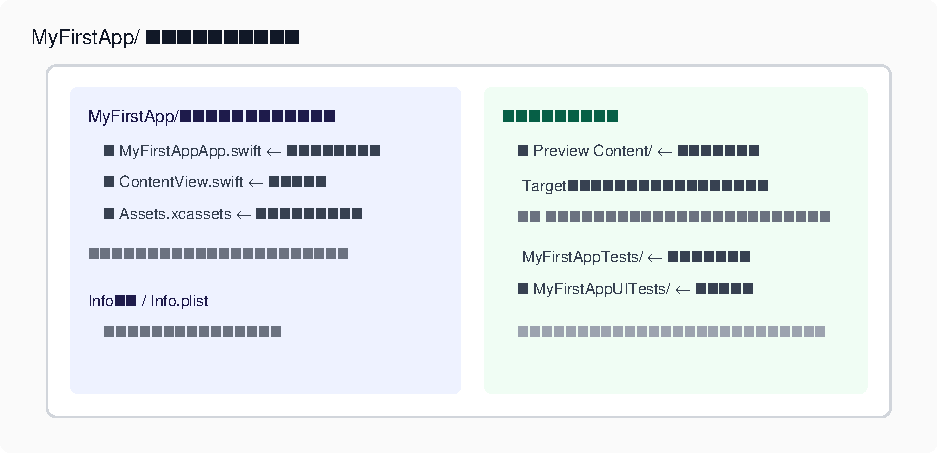
\includegraphics[width=0.92\linewidth]{figures/fig-di-liu-shi-zhang-1}
\\[2pt]\small 図2：初心者が必ず知りたいXcodeのプロジェクト構造
\end{center}

\begin{itemize}
  \item MyFirstAppApp.swift：プログラムの入口。SwiftUIではわずか数行——「起動して、メイン画面を表示する」だけです。
  \item ContentView.swift：メイン画面のビュー。いまあなたが見ているものは、ぜんぶここにあります。
  \item Assets.xcassets：リソースの倉庫——アイコン·画像·色はここに置きます。
  \item Targetの設定：左側の青いプロジェクトアイコンをクリックして入ります。バージョン番号、対応最低iOSバージョン、署名はぜんぶここにあります。アプリの表示名やアイコンもここで設定します。
\end{itemize}

\booksection{実機デバッグ：アプリをあなたのiPhoneに入れる}

\booksection{Xcodeの時短テクニック：初心者に効く「ショートカット裏ワザ」5選}

これを使いこなせば、あなたはグッと「プロっぽく」見えます：

\begin{center}
\begin{tabularx}{\linewidth}{|X|X|X|}
\hline
\textbf{操作} & \textbf{ショートカット} & \textbf{効果} \tabularnewline
\hline
実行 & CmdR & ビルドして動かす \tabularnewline
キャンバスプレビューの表示／切り替え & OptionCmd & 見たままがそのまま出るスイッチ \tabularnewline
インデントを整形 & CtrlI & 選択したコードのインデントを自動で整える \tabularnewline
ファイルをすばやく開く & CmdO & ファイル名を入れて即オープン（いちばん使う！） \tabularnewline
コメント化／コメント解除 & Cmd/ & デバッグ中にコードを手軽にオン·オフする \tabularnewline
\hline
\end{tabularx}
\end{center}

\begin{center}\small\color{gray}Xcodeのよく使うショートカット（初心者の基本5選）\end{center}

さらに2つの隠れた特典：シミュレータの複数起動（iPhoneとiPadを同時に動かしてレイアウトを比較）と、コードスニペット庫（よく使う数行を右側のSnippetsパネルにドラッグしておけば、次からワンクリックで挿入）——効率化ツールはまず使ってみると、手感は自然についてきます。

\booksection{実機デバッグ：アプリをあなたのiPhoneに入れる}

シミュレータも便利ですが、ゴールは実機です。無料のApple IDでも実機デバッグはできます：

\begin{enumerate}
  \item ケーブルでiPhoneをつなぐ（または同じWi-Fiでワイヤレスデバッグ）。
  \item Xcode上部のデバイスリストで自分のiPhoneを選びます。初回はApple IDでのサインインと、署名の自動設定を案内されます。
  \item iPhoneの［設定］［一般］［VPNとデバイス管理］で、開発者証明書を信頼します。
  \item >を押すと、アプリが実機に入ります。
\end{enumerate}

\begin{tcbwarn}{注意：無料アカウントの「7日間制限」}
無料Apple IDで署名したアプリは7日後に使えなくなります（もう一度実行すれば更新されます）。これはAppleの不正利用防止の仕組みで、学習段階なら十分です。有料開発者アカウント（年99ドル）ならこの制限はありません。詳しくは第六十七章で。

\end{tcbwarn}

\booksection{さっそく試す＋よくあるエラーの応急処置}

\booksection{さっそく試す＋よくあるエラーの応急処置}

ContentView.swiftを開いて、Text(“Hello, world!”)の中の文字を自分の名前に変え、CmdRでもう一度実行——数秒後、シミュレータに自分の名前が表示されます。おめでとうございます。「コードを直す ビルド インストール 実行」という、最初の完全なサイクルを終えました。

\begin{center}
\begin{tabularx}{\linewidth}{|X|X|X|}
\hline
\textbf{エラーの症状} & \textbf{よくある原因} & \textbf{対処法} \tabularnewline
\hline
Signingエラー & Teamが未選択、証明書の期限切れ & Target Signingで自分のアカウントにチェック。無料アカウントならもう一度実行 \tabularnewline
シミュレータが真っ暗／開かない & イメージが壊れている & メニューのDevice Erase All Content。またはシミュレータを削除して作り直す \tabularnewline
Xcodeのダウンロードが遅い／インストールできない & App Storeのネットワーク不安定 & 時間帯を変える。またはApple開発者サイトから.xipオフラインパッケージをダウンロード \tabularnewline
\hline
\end{tabularx}
\end{center}

\begin{center}\small\color{gray}初心者の環境エラー応急処置表\end{center}

\begin{tcbpractice}{やってみよう：「開発の儀式」リストを完成させる}
(1)Xcodeを入れてシミュレータを動かす。(2)実機で自分のアプリを1回実行し、スクリーンショットを記念に残す。(3)Helloの文字を自分の名前に変える。(4)Target設定でアプリの表示名を「わたしの初めてのアプリ」に変える。この4ステップを終えれば、あなたはもう「作品を持つ人」です。

\end{tcbpractice}

\begin{tcbsummary}{本章のまとめ}
\begin{itemize}
  \item ハードル：Mac＋Xcode。Macがなければ、まずiPadのSwift Playgroundsで言語を学ぶ
  \item XcodeはApp Storeから。新バージョンは新しいOSを求めるので、更新はサボらない
  \item 新規プロジェクトの5要素：名前、Team、Organization Identifier、SwiftUI、Swift
  \item プロジェクトの合言葉：コードはみんなMyFirstApp/フォルダの中。Target設定がバージョンと署名を担当
  \item 無料Apple IDの実機デバッグには7日間の署名制限。有料アカウントなら制限なし
  \item 開発の毎日＝コードを直す CmdR 結果を見る、の繰り返し
\end{itemize}

\end{tcbsummary}
